\documentclass{article}

% citations
\usepackage[numbers]{natbib}   % omit 'round' option if you prefer square brackets
\bibliographystyle{apalike}

\usepackage{blindtext}
\usepackage{lipsum}

% General packages
\usepackage[english]{babel}
\pagenumbering{arabic}
\usepackage{color}
\usepackage{lettrine}
\usepackage{setspace}
\usepackage{yfonts}
\usepackage{type1cm}

% Graphics packages
\usepackage{graphicx}
\usepackage{rotating}
% figures
\usepackage{subcaption}

% Math
\usepackage{array}
\usepackage{amsmath}
\usepackage{amsfonts}
\usepackage{amssymb}
\usepackage{geometry}
\usepackage{xparse}
\usepackage{physics}

% Problem environment
\newenvironment{problem}[2][Problem]{\begin{trivlist}
\item[\hskip \labelsep {\bfseries #1}\hskip \labelsep {\bfseries #2.}]}{\end{trivlist}}

\usepackage{xspace}
\newcommand{\A}{\ensuremath{\mathcal{A}}\xspace}
\newcommand{\B}{\ensuremath{\mathcal{B}}\xspace}
\newcommand\pa[1]{\ensuremath{\left(#1\right)}}

\begin{document}

\title{Problem Set 1}
\author{Kara Jones \\
ECON833: Computational Methods for Economists}
\date{Fall 2021}
\maketitle


    \paragraph{Introduction} 
       \paragraph {}Kingstree, South Carolina is a small town in South Carolina that is thirsty for economic development. 
    It was the only town I visited during my internship at the Department of Commerce, and yet it made a lasting impression.
    The town was quiet, ghostly, as though all of the habitants had run out as soon as the government rolled up in their white van. 
    We were greeted by the economic developer and the mayor, both who assured us that they were thrilled to have us visit even though the town didn't show the same excitement.
    Our time in Kingtree, South Carolina was limited, but it left a heavy feeling on my heart.
    The mayor described the town as in danger of dying if additional economic development did not reach its borders.
    Yet when we drove around the town, it also appeared that Kingtree had little to offer.
    While there was plenty of land to built, the infrastructure was lacking, there wasn't an educated workforce, and the rural town couldn't attract a talented workforce to its land either.
    It seemed as though Kingstree, South Carolina was sunk. \par
        Three years later, I visited another small town with little resources and a small educated workforce. 
    Like Kingstree, SC, this community had a problem where their young workforce would leave the town in order to pursue better career opporuntities elsewhere. 
    But unlike Kingstree, the people left in this small town were anything but poor. 
    In fact, they lived in a town with one of the highest GDPs per capita in the world. 
    This tiny town was in a microstate, the six smallest country in the world, the co-principality of Andorra. 
    Many problems that Kingstree faced, the lingering effects could be seen in Andorra as well. 
    Working in the education system, I experienced many of these items firsthand.
    However, Andorra had two things that Kingstree lacked: a thriving tourism economy and tax haven status. \par
        Since these two adventures I had, I've been intrigued by the question: can what makes Andorra thrive be replicated in our poor communities in the US?
    Can tourism and tax-haven status help bring communities out of an endless cycle of poverty and offer more opportunity?
    From these question stem my PhD research interests. 

    \paragraph*{Research Interests}   \par
   \paragraph{} Throughout the PhD program, I'd like to focus my PhD research on the following topics and questions:
    \begin{itemize}
        \item Impact of Economic Incentives in Poor Communities - Do the benefits of economic incentives justify the costs?
        \item Tourism and Tax Haven Status in Micro States - Can these attributes help poor America?
        \item Impact of Free College on Tuition Rates - How do full funded higher education initiatives affect the price of higher education degress?
    \end{itemize}

\paragraph*{Topic 1: Impact of Economic Incentives in Poor Communities}
\paragraph{}Economic incentives are special policies that federal, state, and local governments implement to attract business and encourage investment in a geographical area of interest. 
They are highly contested because of the lack of research showing how the money spent by the government produces economic output and increased standard of living for its inhabitants.
Since the money for economic incentives comes from taxes, it's important that research exists to justify the expense and educate other development organizations on how incentives can be leveraged to boost economic development.
It would be also interesting to explore how the impact of economic incentives compare to other factors in alleviating poverty.
For example, a study by \Citeauthor{fuwa2007pathways} in the Philippines based on 30 years of data showed that determinants of economic mobility and their importance changed over time (Figure \ref{fig:econmobil}) [\cite{fuwa2007pathways}]. \\

\begin{figure}[!h]
    \centering
    \begin{minipage}{0.6\textwidth}
        \centering
        \caption{Upward Mobility Probabilities}
        \label{fig:econmobil}
        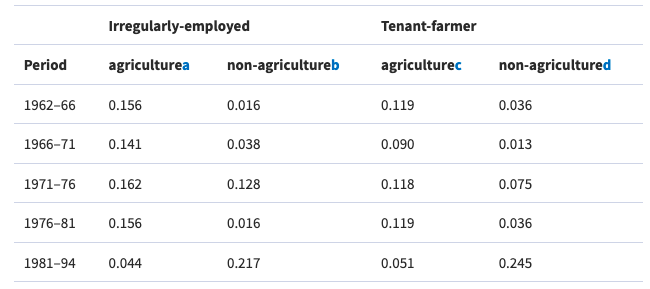
\includegraphics[scale=.4]{econmobil.png}
    \end{minipage} \hspace{0.5cm}
    \end{figure}
    \textit{Source: Household censuses collected by James N. Anderson and \Citeauthor{fuwa2007pathways}.} \cite{fuwa2007pathways}.
    \paragraph*{Topic 2: Tourism and Tax Haven Status in Micro States}
      \paragraph{}  Tourism is a lucrative industry, and people are starting to notice.
   In a 2018 study, tourism was found to produce \$ 3.2 more in GDP across the economy for every dollar spent in tourism \citenum{bode2018benchmarking}.
    Microstates in particular are looking to tourism as the crux of the economic development strategy \cite{bishop2010tourism}. 
    In the study, \Citeauthor{bishop2010tourism} analyzes how St. Lucia and St. Vincent use tourism in different ways to spur economic development.
    His analysis concludes that St. Lucia has more success than its counterpart because of the framework it set up at the inception of the intiative.
    Using similar data from a rural area in the US, I'd like to ascertain if tourism or a tax haven status has improved poverty rates and economic output in the aforementioned community.
    However, Bishop also suggests that the addition of tourism as a prime industry could have ramifications on the social and economic landscapes [\citenum{bishop2010tourism}].
    \pagebreak
    \paragraph*{Topic 3: Impact of Free College on Tuition Rates} 
       \paragraph{}An important factor to consider with economic development is education as one of the fundamental inputs in a business is labor.
    Whether the business runs a call center, a manufacturing plant, a fufilment warehouse, or a storefront, these business must be properly staffed in order to operate.
    Workforce Training Development programs have become hallmarks of quality economic development organizations. 
    They have realized that attracting businesses to their region requires more than available land and sufficient infrastructure. 
    Having a talented workforce already in place to work in business facility's contribute to a region's attractiveness as a business destination.
        Through higher education, people gain skills and knowledge that equips them to work in a variety of career fields. 
    States such as Georgia, South Carolina, and California offer grants to students that cover tuition or a significant portion of tuition for state-funded schools.
    These grants are offered with restrictions such as a minimum GPA, standardized test score, and continued good academic standing.
    While on paper, these tuition grants seem to offer hard-working students an opportunity to go to university, I also anticipate that these grants are also driving up the cost of college tuition.

    \begin{equation} \label{eqn:profit}
        P = T_t - C_e
        \end{equation}

        \begin{equation} \label{eqn:p_detail}
        P = Q_1 \beta_1 + Q_1 \gamma_1 - Q_1 C_s 
    \end{equation}


   In essence, these tuition grants are government subsidies, and thus encourage or discourage an entity from partaking in an activity. 
    With regards to university tuition, government subsidies encourage students to pursue a four-year college degree at a state-funded institution. 
    My hypothesis is that indirectly, these subsidies also encourage universities to accept more students and raise prices.
 See Equations above (\ref{eqn:profit}) and (\ref{eqn:p_detail}).

Tuition rates can be raised in order to exhaust the student's buying power and capture the surplus of the government subsidy. 
The FASFA program fosters price discrimination by the university that allows the university to charge more out of pocket from wealthier students and less from lower-income students.\\
    Other education models, such as those in Andorra and Germany, offer higher education at universities as well as in trade schools and technical colleges.
    Instead of having duplicated programs at each school, the schools are specialized and develop their expertise in a specific field, such as business or computer science.
    By reducing waste in the higher education system and offering degrees at different levels, these countries can offer free tuition at a lower cost than the United States.
    With this type of research, I'd like to encourage education policy in the United States to invest in alternative education models instead of pushing everyone to go to a four-year university.


\bibliography{bibliography}


\end{document}